
\section{杂项选项}
\label{sec:pgfplots:misc}

\begin{pgfplotskey}{disablelogfilter=\mchoice{true,false} (initially false, default true)}
    禁用 \TeX{} 中 $\log(x)$ 的数值求值。如果指定此选项，任何绘图坐标和刻度位置必须以 $\log(x)$ 而非 $x$ 提供。这可能比数值对数更快且（可能）更准确。$\log(x)$ 的当前实现将~$x$ 规范化为 $m\cdot 10^e$ 并计算
        \[
            \log(x) = \log(m) + e \log(10)
        \]
    其中 $y = \log(m)$ 使用应用于 $\exp(y) - m$ 的牛顿法计算。规范化涉及字符串解析，不使用 \TeX{} 寄存器。你可以安全地求值 $\log(1\cdot 10^{-7})$，尽管 \TeX{} 寄存器对此类小数会产生下溢。
\end{pgfplotskey}

\begin{pgfplotskey}{disabledatascaling=\mchoice{true,false} (initially false, default true)}
\label{pgfplots:disabledatascaling}
        \index{Accuracy!Data Transformation}%
        \index{Errors!dimension too large}%
    禁用输入数据的内部重新缩放。通常，每个输入数据（如绘图坐标、刻度位置等）都在不使用 \TeX{} 有限数字精度的情况下解析。然后，将类似
        \[ T(x) = 10^{q-m} \cdot x - a \]
    的变换应用于每个输入坐标/位置，其中 $m$ 是以~$10$ 为底的“$x$ 的阶”。示例：$x=1234 = 1.234\cdot 10^3$ 的阶为~$m=4$，而 $x=0.001234 = 1.234\cdot 10^{-3}$ 的阶为 $m=-2$。参数~$q$ 是坐标轴宽/高的阶。

    该变换的\textbf{效果}是你的绘图坐标可以具有\emph{任意大小}，如 $0.0000001$ 和 $0.0000004$。对于这两个坐标，\PGFPlots{} 在内部将使用 100pt 和 400pt。该变换相当快，因为它仅依赖于周期移位。这种缩放允许超出 \TeX{} 能力的精度。
%    \footnote{Please note that while plot coordinates can be of quite large
%    magnitude like $10^12$ or $10^{-9}$, \PGFPlots{} still uses
%    \TeX{} registers internally (the math parser of \PGF). If your axis
%    interval is $[1234567.8, 1234567.9]$ or something like that.}

    选项“|disabledatascaling|”禁用此数据变换。这有两个后果：首先，坐标表达式如 \parg{{\normalfont\texttt{axis cs:}}x,y} 与 \parg{x,y} 具有相同效果，不应用重新缩放。其次，坐标被限制为 \TeX{} 可以处理的范围。\footnote{请注意，坐标轴缩放需要计算 $1/( x_{\max} - x_{\min} )$。选项 \protect\pgfmanualpdfref{disabledatascaling}{\texttt{disabledatascaling}} 在此上下文中可能导致上溢或下溢，请谨慎使用！通常，数据缩放变换避免此问题。}

    到目前为止，数据缩放变换仅适用于普通坐标轴（对数刻度不需要它）。
\end{pgfplotskey}

\begin{pgfplotskey}{execute at begin plot=\marg{commands}}
    此坐标轴选项允许在每个 |\addplot| 命令的开头调用 \meta{commands}。参数 \meta{commands} 可以是任何 \TeX{} 内容。

    你可以将其与 |x filter=...| 结合使用以重置任何计数器等。一个示例是更改每第 $4$ 个坐标。
\end{pgfplotskey}

\begin{pgfplotskey}{execute at end plot=\marg{commands}}
    此坐标轴选项允许在每个 |\addplot| 命令之后调用 \meta{commands}。参数 \meta{commands} 可以是任何 \TeX{} 内容。
\end{pgfplotskey}

\begin{pgfplotskey}{execute at begin axis=\marg{commands}}
    允许在 |\begin{axis}|（或其他“begin axis”语句）的末尾调用 \meta{commands}。

    该语句作为准备完成之前（几乎）最后的语句执行。
\end{pgfplotskey}

\begin{pgfplotskey}{execute at end axis=\marg{commands}}
    |execute at begin axis| 的对应项。该钩子实际上是多余的，它在 |before end axis| 之后立即执行。它与 |execute at begin axis| 在同一个 \TeX{} 组中执行。
\end{pgfplotskey}

\begin{pgfplotskey}{execute at begin plot visualization=\marg{commands}}
    允许添加自定义代码，该代码在每次绘图可视化的开头执行。与 |execute at begin plot| 不同，这不是在 |\addplot| 期间立即发生，而是在 |\end{axis}| 的后处理后期、生成实际绘图命令时发生。

    下面展示一个可能的应用：\footnote{这个来自博弈论的示例由 Pavel St\v r\'\i \v z 提供。}假设你想使用 |\usepackage{ocg}| 以便动态切换图层，例如在 beamer 包中。这可以如下实现：
    %
% \usepackage[pdftex]{pgfplots_ocg_copy}
\begin{codeexample}[]
% requires \usepackage[pdftex]{ocg}
\begin{tikzpicture}
    \begin{axis}[
        title=Dynamic PDF Layer Support (see Acrobat Layers),
        view={110}{35},
    ]
        \addplot3+ [
            execute at begin plot visualization=\begin{ocg}{First Layer}{FirstLayer}{0},
            execute at end plot visualization=\end{ocg},
        ]
            coordinates {(0,0,12) (0,1,2) (1,0,6) (0,0,12)};

        \addplot3+ [
            execute at begin plot visualization=\begin{ocg}{Second Layer}{SecondLayer}{0},
            execute at end plot visualization=\end{ocg},
        ]
            coordinates {(0,0,9) (0,1,8) (1,0,4) (0,0,9)};

        \addplot3+ [
            execute at begin plot visualization=\begin{ocg}{Third Layer}{ThirdLayer}{0},
            execute at end plot visualization=\end{ocg},
        ]
            coordinates {(0,0,1) (0,1,7) (1,0,3) (0,0,1)};
    \end{axis}
\end{tikzpicture}
\end{codeexample}
    %
    \noindent |execute *| 钩子在正确位置插入 \textsc{ocg} 语句，单个绘图命令被添加到不同的动态图层。使用 Acrobat Reader 及其“图层”选项卡来打开或关闭每个图层。请注意，仅将 |\begin{ocg}...| 语句直接添加到文本中是不够的，因为 \PGFPlots{} 将绘图命令推迟到 |\end{axis}|（勘察阶段和可视化阶段的分离）。

    有关 \textsc{ocg} 及其获取方式的更多详细信息，请参见 \url{http://www.texample.net/weblog/2008/nov/02/creating-pdf-layers}。

    技术说明：这些钩子也会为 |\pgfplotsextra| 命令插入。
\end{pgfplotskey}

\begin{pgfplotskey}{execute at end plot visualization=\marg{commands}}
    这是 |execute at begin plot visualization| 的对应项。
\end{pgfplotskey}

\begin{pgfplotskey}{forget plot=\marg{true,false} (initially false)}
\label{pgfplots:forgetplot}
    允许包含不会被记住用于图例条目、不会增加绘图数量、且不会被循环列表考虑的图。

    被遗忘的图可以是某种装饰，它具有单独的样式且不影响坐标轴状态，尽管它像任何其他图一样被处理。如下例所示，将此选项提供给 |\addplot|。
    %
\begin{codeexample}[]
\begin{tikzpicture}
\begin{loglogaxis}[
    % some descriptions:
    table/x=Basis,
    table/y={L2/r},
    xlabel=Degrees of Freedom,
    ylabel=relative Error,
    title=New Experiments (old in gray),
    legend entries={$e_1$,$e_2$,$e_3$},
]
    \addplot [black!15,forget plot]
        table {plotdata/oldexperiment1.dat};
    \addplot [black!15,forget plot]
        table {plotdata/oldexperiment2.dat};
    \addplot [black!15,forget plot]
        table {plotdata/oldexperiment3.dat};
    \addplot table {plotdata/newexperiment1.dat};
    \addplot table {plotdata/newexperiment2.dat};
    \addplot table {plotdata/newexperiment3.dat};
    \end{loglogaxis}
\end{tikzpicture}
\end{codeexample}
    %
    由于被遗忘的图不会增加绘图索引，它们将使用与后续图相同的 |cycle list| 条目。

    样式 |every forget plot| 可用于配置每个此类图的样式：
    %
\begin{codeexample}[]
\begin{tikzpicture}
\begin{loglogaxis}[
    forget plot style={opacity=0.2},
    % same as above:
    table/x=Basis,
    table/y={L2/r},
    xlabel=Degrees of Freedom,
    ylabel=relative Error,
    title=New Experiments (old in transparent),
    legend entries={$e_1$,$e_2$,$e_3$},
]
    \foreach \exp in {1,2,3} {
      \addplot+ [forget plot]
          table {plotdata/oldexperiment\exp.dat};
      \addplot table {plotdata/newexperiment\exp.dat};
    }
\end{loglogaxis}
\end{tikzpicture}
\end{codeexample}
    %
    \noindent 这里，|\addplot+| 命令意味着我们使用与后续图相同的 |cycle list|，并且 |forget plot style| 修改 |every forget style|，产生“旧实验”的透明度。

    请注意，|every axis plot no |\meta{index} 样式不适用于此处。

    如果启用了 |stack plots|，被遗忘的图将正常堆叠！
\end{pgfplotskey}

\begin{pgfplotscodekey}{before end axis}
    允许在坐标轴结束之前插入 \meta{commands}（另见 |execute at end axis|）。此选项在裁剪区域内部生效。
    %
\begin{codeexample}[]
\pgfplotsset{
    every axis/.append style={
        before end axis/.code={
            \fill [red] (1,10) circle(5pt);
            \node at (-4,10)
                {\large This text has been inserted
                 using \texttt{before end axis}.};
        },
    },
}
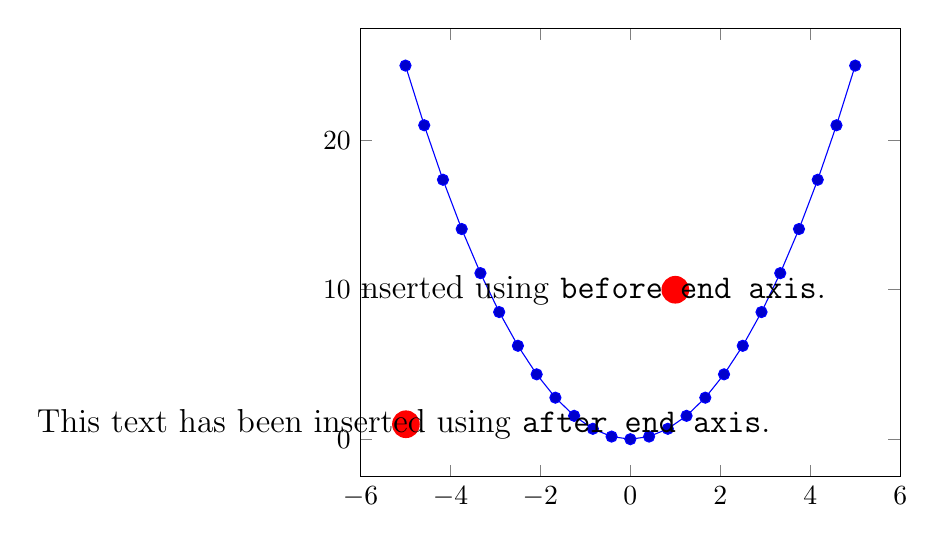
\begin{tikzpicture}
    \begin{axis}
        \addplot {x^2};
    \end{axis}
\end{tikzpicture}
\end{codeexample}
\end{pgfplotscodekey}

\begin{pgfplotscodekey}{after end axis}
    允许在裁剪绘图命令结束之后立即插入 \meta{commands}。虽然 |before end axis| 的效果与将 \meta{commands} 放置在坐标轴内部相同，但 |after end axis| 允许访问坐标轴坐标而不被裁剪。
    %
\begin{codeexample}[]
\pgfplotsset{
    every axis/.append style={
        after end axis/.code={
            \fill [red] (1,10) circle(5pt);
            \node at (-4,10)
                {\large This text has been inserted using \texttt{after end axis}.};
        },
    },
}
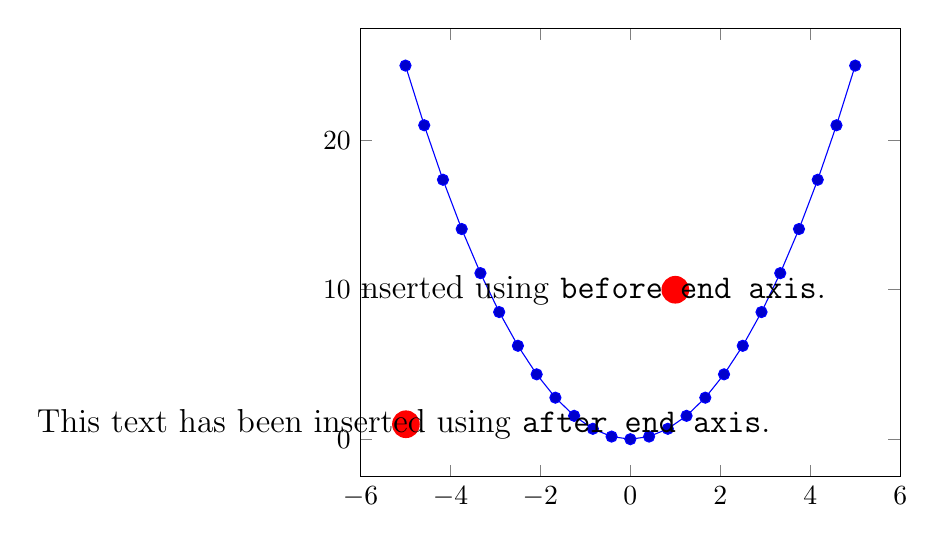
\begin{tikzpicture}
    \begin{axis}
        \addplot {x^2};
    \end{axis}
\end{tikzpicture}
\end{codeexample}
\end{pgfplotscodekey}

\begin{pgfplotskey}{axis on top=\mchoice{true,false} (initially false)}
    如果设置为 |true|，坐标轴线、刻度、刻度标签和网格线将绘制在绘图图形之上。
    %
\begin{codeexample}[]
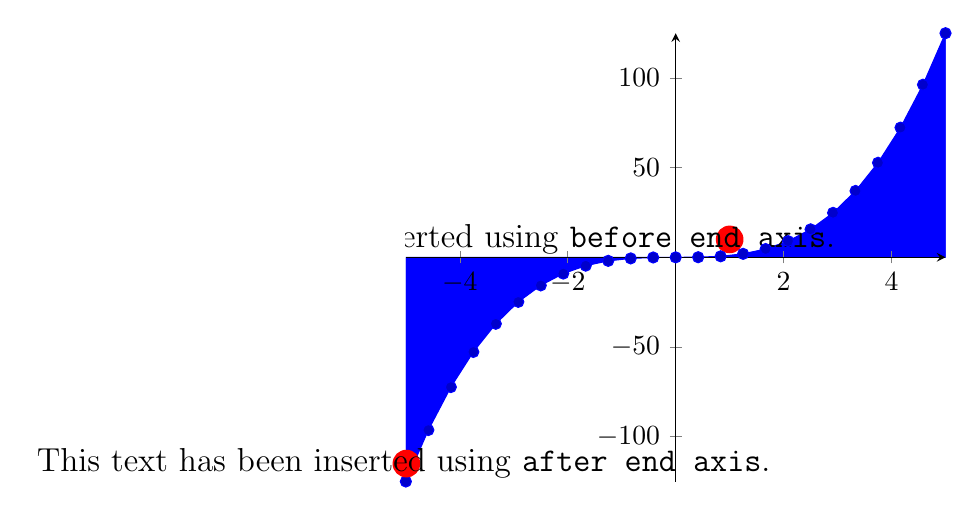
\begin{tikzpicture}
\begin{axis}[
    axis on top=true,
    axis x line=middle,
    axis y line=middle,
]
    \addplot+ [fill] {x^3} \closedcycle;
\end{axis}
\end{tikzpicture}
\end{codeexample}

\begin{codeexample}[]
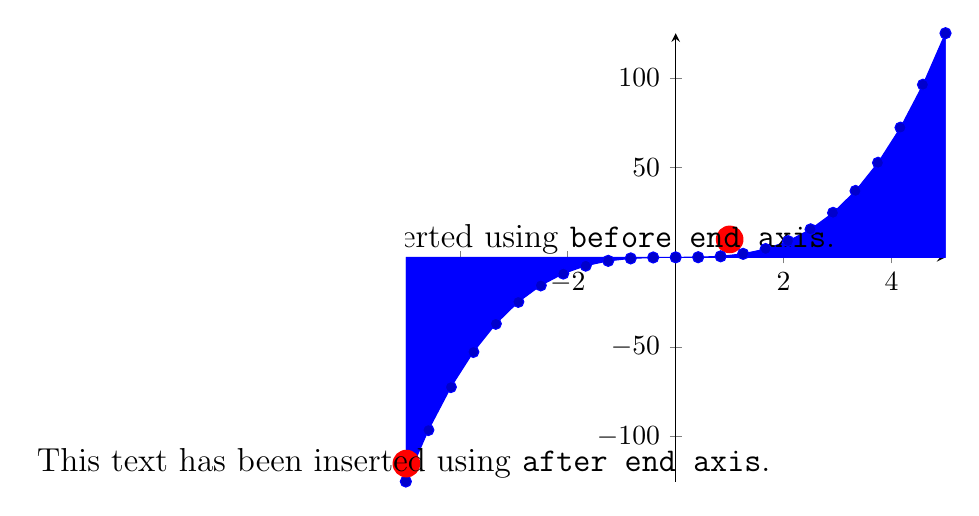
\begin{tikzpicture}
\begin{axis}[
    axis on top=false,
    axis x line=middle,
    axis y line=middle,
]
    \addplot+ [fill] {x^3} \closedcycle;
\end{axis}
\end{tikzpicture}
\end{codeexample}
    %
    请注意，此功能不影响绘图标记。我认为如果绘图标记被坐标轴描述穿过，看起来会不熟悉。
\end{pgfplotskey}

\begin{pgfplotskeylist}{%
    visualization depends on=\meta{\textbackslash macro} (initially empty),%
    visualization depends on=\meta{expression}\texttt{\textbackslash as}\meta{\textbackslash macro} (initially empty),
    visualization depends on=\texttt{value }\meta{content}\texttt{\textbackslash as}\meta{\textbackslash macro} (initially empty)%
}
    允许向 \PGFPlots{} 传达数据，这些数据对于执行可视化至关重要，尽管 \PGFPlots{} 不知道它。

    假设你想要一个散点图，它依赖于 $(x,y)$ 坐标、用于绘制单独颜色的 |point meta| 数据，以及影响 |mark size| 的数据。因此，每个数据点总共需要~$4$ 个坐标，尽管 \PGFPlots{} 在其初始配置中仅支持 $3$ 个。

    在我们真正谈到问题的要点之前，我们先谈谈如何获得一个具有单独颜色\emph{和}单独大小的散点图。仅设置 |mark size| 是不够的，因为 |mark size| 只在处理标记之前求值一次（|every mark| 也是如此）。因此，我们可以使用 |scatter| 结合

    |scatter/@pre marker code/.append style={/tikz/mark size=\perpointmarksize}|.

    \noindent |@pre marker code| 为散点图的每个标记单独安装。现在，我们谈到问题本身：我们从哪里获得 |mark size| 的值，在我们的案例中称为 |\perpointmarksize|？

    一个解决方案是 |visualization depends on|（此处使用第二种输入语法）：
    %
\begin{codeexample}[]
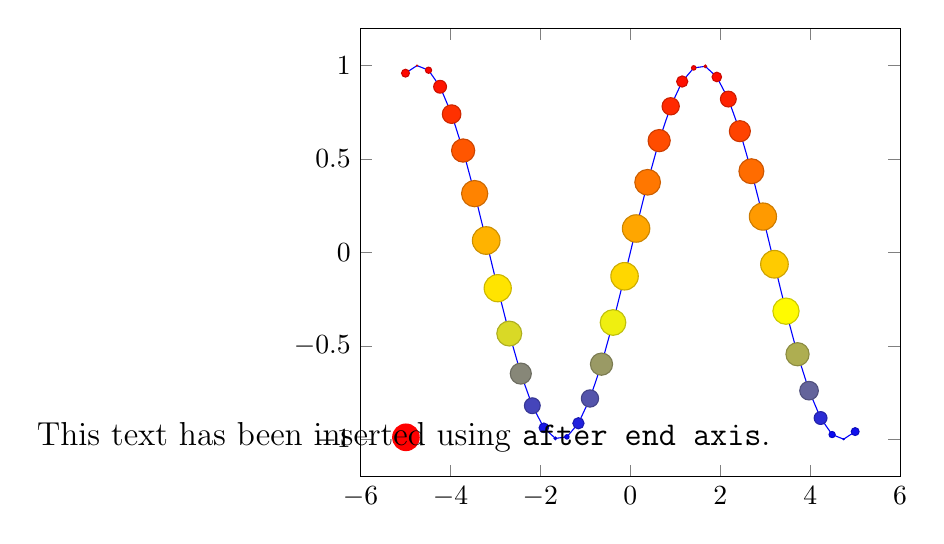
\begin{tikzpicture}
\begin{axis}
    \addplot+ [
        scatter,
        scatter src=y,
        samples=40,
        visualization depends on=
            {5*cos(deg(x)) \as \perpointmarksize},
        scatter/@pre marker code/.append style=
            {/tikz/mark size=\perpointmarksize},
    ]
        {sin(deg(x))};
\end{axis}
\end{tikzpicture}
\end{codeexample}

    这里，我们将 |\perpointmarksize| 定义为 |5*cos(deg(x))|。该表达式将与所有其他坐标一起求值。因此，勘察阶段可用的一切都可以在此使用。这包括最终坐标 |x|、|y|、|z|；常量 |meta| 展开为当前逐点元数据。此外，|\thisrow|\marg{colname} 展开为表格列的值。

    命令 |visualization depends on| 求值并记住内部数据结构中的每个值。记住的值在可视化阶段作为 \meta{\textbackslash macro} 可用。在我们的示例中，|@pre marker code| 在可视化阶段求值并应用 |mark size=5*cos(deg(x))|。

    第一种语法 |visualization depends on=|\meta{\textbackslash macro} 告诉 \PGFPlots{} 使用已定义的 \meta{\textbackslash macro}。第二种语法带有 \meta{content}|\as|\meta{\textbackslash macro} 也提供值。

    可以有不止一个 |visualization depends on| 短语。

    如果存储的值不是数值类型，\footnote{或者如果它只是一个常量而你想提高速度。}你可以在参数前使用前缀 `|value|'，即

    |visualization depends on=value |\meta{\textbackslash macro} 或

    |visualization depends on=value |\meta{content}|\as |\meta{\textbackslash macro}.

    这样的值将被展开并存储，但不会被解析为数字（至少不由 \PGFPlots 解析）。
\end{pgfplotskeylist}

\begin{key}{/pgf/fpu=\marg{true,false} (initially true)}
        \index{Precision}
    此键启用或禁用浮点单元。如果它被禁用（|false|），由 Mark Wibrow 和 Till Tantau 编写的核心 \PGF{} 数学引擎将用于 |\addplot expression|。然而，此引擎是为生成图形而编写的，不适合科学计算。它限于范围 $\pm 16384.00000$ 内的定点数。

    如果 |fpu| 被启用（|true|，初始配置），将使用由 Christian Feuers\"anger 编写的 \PGF{} 高精度浮点库。它在 \TeX{} 中提供完整范围的 IEEE 双精度计算。此 FPU 也是 \PGFPlotstable{} 的一部分，并且默认对 |create col/expr| 和所有其他预定义数学方法启用。

    使用
    %
\begin{codeexample}[code only]
\pgfkeys{/pgf/fpu=false}
\end{codeexample}
    \noindent 以停用扩展精度。如果你更喜欢使用 |fp|（定点）包，可能结合 Mark Wibrow 相应的 \PGF{} 库，|fpu| 将自动停用。然而，请注意 |fp| 的数据范围较小（约 $\pm 10^{17}$），并且可能更慢。
\end{key}
